\documentclass{article}
\usepackage[utf8x]{inputenc}
\usepackage{ucs}
\usepackage{amsmath} 
\usepackage{amsfonts}
\usepackage{upgreek}
\usepackage[english,russian]{babel}
\usepackage{graphicx}
\usepackage{float}
\usepackage{textcomp}
\usepackage{hyperref}
\usepackage{geometry}
  \geometry{left=2cm}
  \geometry{right=1.5cm}
  \geometry{top=1cm}
  \geometry{bottom=2cm}
\usepackage{tikz}
\usepackage{ccaption}
\usepackage{multicol}

\usepackage{listings}
%\setlength{\columnsep}{1.5cm}
%\setlength{\columnseprule}{0.2pt}


\begin{document}
\pagenumbering{gobble}

\lstset{
  language=C,                % choose the language of the code
  basicstyle=\linespread{1.1}\ttfamily,
  columns=fixed,
  fontadjust=true,
  basewidth=0.5em,
  keywordstyle=\color{blue}\bfseries,
  commentstyle=\color{gray},
  stringstyle=\ttfamily\color{orange!50!black},
  showstringspaces=false,
  %numbers=false,                   % where to put the line-numbers
  numbersep=5pt,
  numberstyle=\tiny\color{black},
  numberfirstline=true,
  stepnumber=1,                   % the step between two line-numbers.        
  numbersep=10pt,                  % how far the line-numbers are from the code
  backgroundcolor=\color{white},  % choose the background color. You must add \usepackage{color}
  showstringspaces=false,         % underline spaces within strings
  captionpos=b,                   % sets the caption-position to bottom
  breaklines=true,                % sets automatic line breaking
  breakatwhitespace=true,         % sets if automatic breaks should only happen at whitespace
  xleftmargin=.2in,
  extendedchars=\true,
  keepspaces = true,
}
\lstset{literate=%
   *{0}{{{\color{red!20!violet}0}}}1
    {1}{{{\color{red!20!violet}1}}}1
    {2}{{{\color{red!20!violet}2}}}1
    {3}{{{\color{red!20!violet}3}}}1
    {4}{{{\color{red!20!violet}4}}}1
    {5}{{{\color{red!20!violet}5}}}1
    {6}{{{\color{red!20!violet}6}}}1
    {7}{{{\color{red!20!violet}7}}}1
    {8}{{{\color{red!20!violet}8}}}1
    {9}{{{\color{red!20!violet}9}}}1
}

\title{Семинар \#1: Работа с командной строкой. Основы C. \vspace{-5ex}}\date{}\maketitle
\section*{Часть 1: Работа с командной строкой:}
\subsection*{Основные команды:}
\texttt{
\begin{tabular}{ c | c }
 pwd                     & напечатать имя текущей директории \\ 
 ls                      &  напечатать все файлы и папки текущей директории \\ 
 ls -l                   &  то же, что и ls, но больше информации о файлах \\
 cd <имя папки>          & перейти в соответствующую папку \\
                         & например:  cd /home-local/student \\
 mkdir <имя новой папки> & создать новую папку \\
 cp <путь до файла> <путь до копии> & скопировать файл \\
 mv <путь до файла> <новый путь>    & переместить или переименовать файл  \\
 rm <путь до файла>                 & удалить файл \\
 rm -r <путь до папки>              & удалить папку \\
\end{tabular}
}




\subsection*{Компилятор \texttt{gcc}:}
\texttt{
\begin{tabular}{ c | c }
 gcc <имя файла исходного кода>  & скомпилировать программу и создать исполняемый файл \texttt{a.out} \\ 
                                 & файл исходного кода должен иметь расширение \texttt{.c} \\
 <путь до исполняемого файла>    & запустить исполняемый файл \\
 ./a.out                         & например, запустить файл a.out в текущей директории \\ 
                                 & . - текущая директория; a.out - имя файла \\ 
 gcc -o <исполняемый файл> <.c файл>  & скомпилировать программу и создать исполняемый файл \\
 gcc -std=c11 <.c файл>  & использовать стандарт языка C 2011-го года \\
 gcc -lm <.c файл>  & подключить математическую библиотеку (если вы используете math.h) \\
\end{tabular}
}
\\
\begin{center}
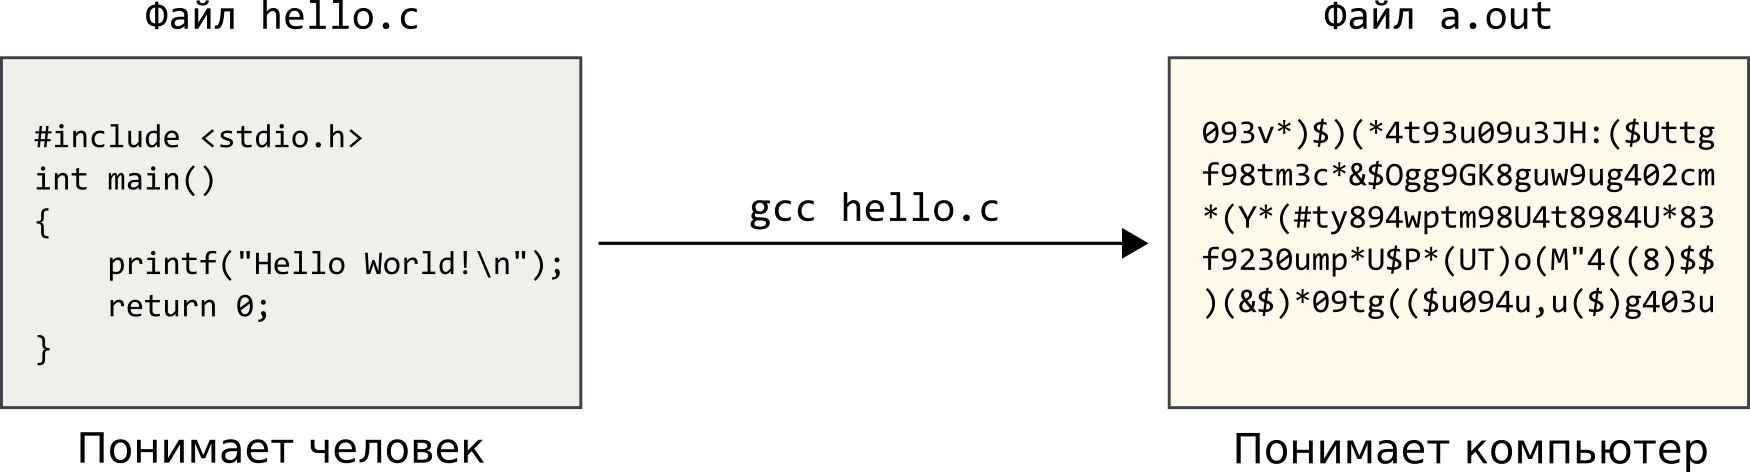
\includegraphics[scale=1]{../images/gcc_simple.png}
\end{center}

\subsection*{Сокращение директорий:}
\texttt{
\begin{tabular}{ c | c }
 /                       & корневая директория \\ 
 .                       & текущая директория \\ 
 ..                      & директория, которая содержит текущую \\ 
 \texttildelow                       & директория пользователя (/home-local/student) \\
\end{tabular}
}

\subsection*{Горячие клавиши:}
\texttt{
\begin{tabular}{ c | c }
 Tab           & автозаполнение \\ 
 2 раза Tab    & показать возможные варианты \\ 
 стрелка вверх & перейти к предыдущей команде \\ 
 Ctrl-C        & выход из программы, например той, которая зависла \\ 
 Ctrl-R        & поиск по всем предыдущим командам \\ 
\end{tabular}
}




\subsection*{Задание на работу с командной строкой:}
\begin{enumerate}
\item Откройте терминал и узнайте в какой папке вы находитесь. Для этого напечатайте \texttt{pwd} и нажмите \texttt{Enter}.
\item Перейдите в папку  \texttt{/home-local/student}. Для этого введите команду:
\begin{verbatim}
cd /home-local/student
\end{verbatim}
\item С помощью команды \texttt{pwd} проверьте, что вы действительно находитесь в нужной папке.
\item С помощью команды \texttt{ls} просмотрите всё содержимое папки \texttt{/home-local/student}.
\item Создайте вашу папку, в которой вы будете работать в течении семестра. Используйте команду:
\begin{verbatim}
mkdir <имя новой папки> 
\end{verbatim}
За место <имя новой папки>  подставьте название вашей папки (треугольные скобки писать не нужно). Желательно, чтобы название содержало только латинские символы без пробелов.
\item С помощью команды \texttt{ls} убедитесь, что ваша папка создалась.
\item Перейдите в вашу созданную папку командой \texttt{cd <имя папки>}.

\item Перейдите в эту папку с помощью файлового менеджера(проводника) и создайте там файл \texttt{test.txt}.
\item Откройте этот файл с помощью любого текстового редактора и напишите в нём что-нибудь.
\item В командной строке введите команду \texttt{ls}, чтобы убедится что в папке содержится единственный файл \texttt{test.txt}. Если этот файл не отображается с помощью \texttt{ls}, то убедитесь, что вы находитесь в нужной папке, используя команду \texttt{pwd}.
\item Скопируйте этот файл в эту же директорию командой
\begin{verbatim}
cp test.txt <имя копии>
\end{verbatim}
\item Убедитесь, что копия создалась. Для этого используёте \texttt{ls} или файловый менеджер.
\item Используя командную строку, создайте новую папку и скопируйте туда файл \texttt{test.txt}
\item Перейдите в созданную вами новую папку: \texttt{cd <имя папки>}.
\item Используйте \texttt{ls}, чтобы просмотреть содержимое этой папки.
\item Выйдите из этой папки (перейдите выше командой:  \texttt{cd ..})
\item Переименуйте файл \texttt{test.txt}. Для этого используёте команду \texttt{mv test.txt <новое имя>}.
\item Удалить созданные файлы и папки в терминале с помощью \texttt{rm}. Обратите внимание, что обычные файлы и папки удаляются по-разному.
\item В файловом менеджере создайте файл \texttt{test.c} и напишите в нём текст программы \textit{hello world}.
\item В терминале проверьте, что этот файл существует командой \texttt{ls}.
\item Скомпилируйте этот файл следующей командой:
\begin{verbatim}
gcc -o hello test.c
\end{verbatim}
После этого в папке создастся новый файл по имени \texttt{hello} (это имя мы указали в опции \texttt{-o}).
\item Запустите файл \texttt{hello} напечатав команду:
\begin{verbatim}
/home-local/student/<ваша папка>/hello
\end{verbatim}
Или просто 
\begin{verbatim}
./hello
\end{verbatim}
\item Можно объединить команды компиляции и запуска:
\begin{verbatim}
gcc -o hello test.c && ./hello
\end{verbatim}
Измените программу так, чтобы она печатала \texttt{Hello MIPT!}, скомпилируйте и запустите программу. \\
\textit{Примечание}: каждый раз вводить эту команду не нужно, можно просто нажать клавишу вверх.

\end{enumerate}


\newpage
\section*{Часть 2: Основы C}
\subsection*{Hello World!}
Простейшая программа на языке C выглядит следующим образом:
\begin{lstlisting}
#include <stdio.h>
int main() {
    printf("Hello world!");
}
\end{lstlisting}

Эта программа печатает на экран строку "Hello world!".
\begin{itemize}
\item \texttt{\#include <stdio.h>}  - включаем библиотеку stdio (standard input/output), которая содержит \texttt{printf}.
\item \texttt{int main() \{ ... \}} - основная функция программы, с неё начинается исполнение любой программы.
\item \texttt{printf("Hello world!");} - печатаем на экран.
\end{itemize}

\subsection*{Задание на основы \texttt{printf}}
\begin{enumerate}
\item Скомпилируйте программу, используя \texttt{gcc} и запустите.
\item В строке функции \texttt{printf()} можно использовать некоторые специальные символы \texttt{\textbackslash n}, \texttt{\textbackslash t} и \texttt{\textbackslash b}. Добавьте эти символы в строку функции \texttt{printf} (в произвольное место) и выясните, что они делают.
\item Напишите программу, которая будет выводить на экран:
\begin{verbatim}
First
    Second
        Third
\end{verbatim}
Используйте 1 вызов функции \texttt{printf}. Для отступов используйте пробелы или знаки табуляции(\texttt{\textbackslash t}).
\end{enumerate}

\subsection*{Целочисленные переменные \texttt{int}:}
В переменных \texttt{int} можно хранить целые числа от $-2^{31}$ до $2^{31} - 1$. ($2^{31}$ примерно равно двум миллиардам)
\begin{lstlisting}
#include <stdio.h>
int main() {
    int a;
    int b = 5;
    a = 3;
    int res = a * b + (b / a);
    printf("Result = %i\n", res);
}
\end{lstlisting}

\begin{itemize}
\item \texttt{int a} - Объявляем, что у нас есть переменная a, которая будет хранить целые числа.
\item \texttt{int b = 5} - Объявляем, что есть переменная b, которая будет хранить целые числа и присваиваем ей 5.
\item \texttt{a = 3} - Присваиваем переменной a число 3.
\item \texttt{res = a * b + (b / a)} - Сохраняем в переменной res результат вычислений.
\item \texttt{printf(``Result = \%i \textbackslash n '', res)} Печатаем, за место спецификатора \texttt{\%i} (сокращение от \texttt{int}) подставится значение переменной.
\end{itemize}
\subsection*{Задание на целочисленные переменные:}
\begin{enumerate}
\item Создайте переменные \texttt{a} и \texttt{b} и присвойте им значения \texttt{a = 26}, а \texttt{b = 7}. Затем:
	\begin{itemize}
	\item Напечатайте на экран число \texttt{a}. Вот так:
		\begin{lstlisting}
		printf("%i\n", a);
		\end{lstlisting}
	\item Напечатайте на экран 2 числа \texttt{a} и \texttt{b}, разделённые пробелом. Вот так:
		\begin{lstlisting}
		printf("%i %i\n", a, b);
		\end{lstlisting}
	\item Напечатайте на экран 2 числа \texttt{a} и \texttt{b} в следующем формате \texttt{(26, 7)}.
		\begin{lstlisting}
		printf("(%i, %i)\n", a, b);
		\end{lstlisting}
	
	\item Напечатайте на экран 2 числа \texttt{a} и \texttt{b} в следующем формате \texttt{[26:7])}.
	\item Напечатайте на экран 2 числа \texttt{a} и \texttt{b} в следующем формате \texttt{(A = 26 and B = 7)}.
	\item Напечатайте на экран сумму чисел \texttt{a} и \texttt{b}.
	\item Напечатайте на экран произведение чисел \texttt{a} и \texttt{b}.
	\item Напечатайте на экран результат целочисленного деления \texttt{a} на \texttt{b}. Используйте оператор: \texttt{a / b}. В результате этой
		операции должно получиться целое число \texttt{3} (так как это операция деления нацело).
	\item Напечатайте на экран остаток деления \texttt{a} на \texttt{b}. Используйте оператор: \texttt{a \% b}. В результате этой
		операции должно получиться целое число \texttt{5}.
	\end{itemize}
\item Пусть \texttt{a = 2147483647} (максимальное возможное значение для \texttt{int}). Напечатайте значение \texttt{a + 1} и \texttt{2a}.
\end{enumerate}

\section*{Адрес и размер переменной:}
\begin{itemize}
\item 1 бит - минимальная единица измерения памяти. В 1 бите может хранится либо \texttt{0} либо \texttt{1}.
\item Вся память делится на ячейки, размером в 8 бит = 1 байт.
\item Все эти ячейки занумерованы, номер ячейки называется адресом.
\item Все переменные содержатся в памяти. Адрес переменной - это адрес первого байта переменной.
\item Чтобы найти адрес переменной, нужно перед ней поставить \texttt{\&}, например, \texttt{\&a}
\item Чтобы найти размер переменной в байтах: \texttt{sizeof(a)}
\item Например, переменная типа \texttt{int} имеет размер 4 байта = 32 бита. Значит в ней может хранится максимум $2^{32}$ значений.
\end{itemize}

\begin{center}
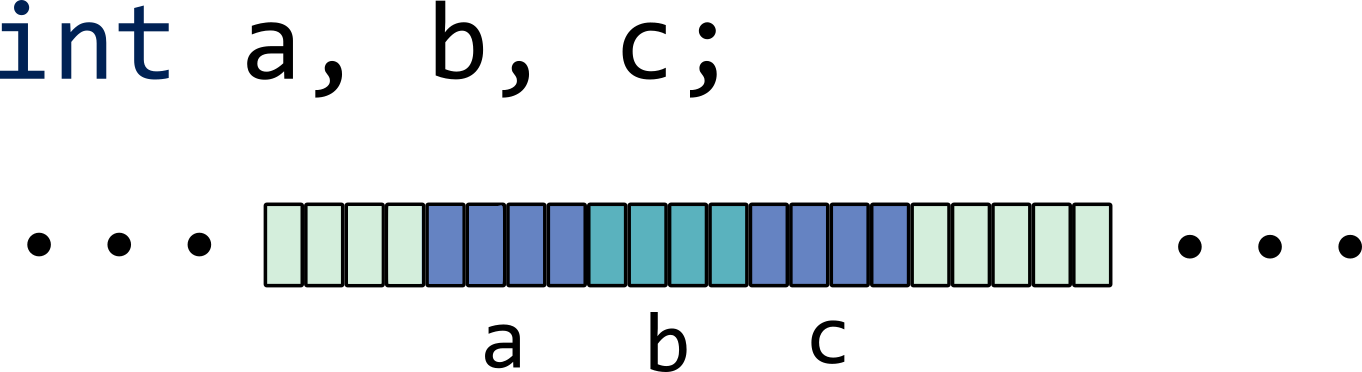
\includegraphics[scale=0.8]{../images/memory_ints.png}
\end{center}

\subsection*{Задание:}
\begin{enumerate}
\item Напечатать размер переменной типа \texttt{int} в байтах. Для этого используйте оператор \texttt{sizeof}:
\begin{lstlisting}
printf("%i\n", sizeof(a));
\end{lstlisting}
\item Напечатать адреса переменных типа \texttt{int}. Для этого используйте оператор \texttt{\&}. Адреса памяти обычно хранятся не в переменных типа \texttt{int}, а в больших по размеру переменных. Поэтому для их печати нужно использовать не \texttt{\%i}, а \texttt{\%lli} или \texttt{\%p}.:
\begin{lstlisting}
printf("%lli %lli\n", &a, &b);
\end{lstlisting}
Убедитесь, что переменные \texttt{a} и \texttt{b} лежат в памяти вплотную друг к другу.
\end{enumerate}

\section*{Считывание переменных - scanf:}
Считывание переменных из терминала осуществляется с помощью функции \texttt{scanf} из библиотеки \texttt{stdio}. В отличии от \texttt{printf}, в \texttt{scanf} нужно передавать не саму переменную, а её адрес. Это естественно, так как \texttt{scanf} должен записать считываемое значение в соответствующие ячейки памяти.\\
Пример программы, которая считывает переменные a и b и печатает на экран их произведение:
\begin{lstlisting}
#include <stdio.h>
int main() {
    int a, b;
    scanf("%i", &a); // <-- не забудьте тут амперсанд &
    scanf("%i", &b); // <-- не забудьте тут амперсанд &
    printf("Result = %i\n", a * b);
}
\end{lstlisting}
\textit{Примечание:} При задании формата в \texttt{scanf} не нужно ставить пробелы и символы переноса строки. Т.е. не нужно писать так:
\begin{lstlisting}
scanf("%i\n", &a);  // будет ожидать ввода ещё одного числа
\end{lstlisting}

\subsection*{Задание на считывание:}
\begin{enumerate}
\item Написать программу, которая считывает целое число и печатает на экран квадрат этого числа.
\item Считать 2 целых числа и напечатать результат целочисленного деления первого на второе. Считать 2 числа с помощью \texttt{scanf} можно и одной строкой: 
\begin{lstlisting}
scanf("%i%i", &a, &b); // <-- не забывайте тут амперсанд &
\end{lstlisting}

\item Считать 2 целых числа и напечатать остаток деления первого на второе.
\item Считать целое число и напечатать его последнюю цифру. Используйте оператор остатка.
\item На вход подаётся прошедшее время в формате \texttt{hh:mm}, например, \texttt{05:14}. Нужно напечатать, общее количество минут (\texttt{314}). Создайте 2 переменные \texttt{hours} и \texttt{minutes} и считать значения этих переменных с помощью \texttt{scanf}. Вот так:
\begin{lstlisting}
scanf("%i:%i", &hours, &minutes); // <-- не забывайте тут амперсанд &
\end{lstlisting}
\end{enumerate}

\section*{Операторы инкремента:}
Для удобства в языке C введены следующие операторы:
\begin{verbatim}
+=    -=    *=    /=     ++   --    и другие
\end{verbatim}
Например оператор присваивания сложения \texttt{+=} увеличивает левый аргумент на величину правого.\\
Оператор \texttt{++} увеличивает значение аргумента на 1.
\begin{lstlisting}
#include <stdio.h>
int main() {
    int a = 100;
    a = a + 5;  // увеличиваем a на 5
    a += 5;     // увеличиваем a на 5 ( то же самое )
    
    a++;        // увеличиваем a на 1
    ++a;        // увеличиваем a на 1
}
\end{lstlisting}
Чему будет равно значение переменной a после выполнение данного кода?


\newpage
\section*{Логические операторы:}
\begin{center}
\texttt{\begin{multicols}{2}
\begin{tabular}{ c c }
 == & равно\\ 
 != & не равно \\  
 > & больше \\  
 >= & больше и равно \\ 
 < & меньше \\
 <= & меньше и равно \\
\end{tabular}
\begin{tabular}{ c c }
 \&\& & логическое И \\ 
 || & логическое ИЛИ \\  
 !  & логическое НЕ \\  
\end{tabular}
\end{multicols}
}
\end{center}

Пример программы, которая считывает возраст человека и печатает \texttt{Yes}, если возраст больше или равен 18:
\begin{lstlisting}
#include <stdio.h>
int main() {
    int age;
    scanf("%i", &age);
    if (age >= 18) {
    	printf("Yes\n");
    }
}
\end{lstlisting}
\quad\\
Пример программы, которая считывает число \texttt{n} и печатает \texttt{Yes}, если число двузначно и \texttt{No} иначе:
\begin{lstlisting}
#include <stdio.h>
int main() {
    int n;
    scanf("%i", &n);
    if (n >= 10 && n < 100) {
       	printf("Yes\n");
    }
    else {
    	printf("No\n");
    }
}
\end{lstlisting}

Пример программы, которая принимает на вход число и печатает \texttt{Positive}, если число положительное, \texttt{Negative}, если число отрицательное и \texttt{Zero}, если число равно нулю:
\begin{lstlisting}
#include <stdio.h>
int main() {
    int n;
    scanf("%i", &n);
    if (n > 0) {
       	printf("Positive\n");
    }
    else if (n == 0){
    	printf("Zero\n");
    }
    else {
    	printf("Negative\n");
    }
}
\end{lstlisting}


\newpage
\subsection*{Задание на логические операторы:}
\begin{enumerate}
\item Написать программу, которая считывает число и печатает \texttt{Yes}, если число равно \texttt{42} и \texttt{No} иначе. Обратите внимание, что для сравнения чисел нужно использовать оператор \texttt{==} ("два равна").
\item Написать программу, которая принимает на вход число и печатает \texttt{Yes}, если число принадлежит множеству $(-\infty, -12] \cup (97, +\infty)$  и \texttt{No} иначе.
\item Написать программу, которая принимает на вход число и печатает \texttt{Even}, если число четное и \texttt{Odd}, если число нечетное. Подсказка: число чётное, если остаток от делениея на 2 равен 0.
\item Написать программу, которая принимает на вход два числа и печатает \texttt{First}, если первое число больше второго, \texttt{Second}, если второе больше первого и \texttt{Equal}, если числа равны.
\item Написать программу, которая принимает на вход два числа и печатает большее из этих двух чисел.
\item Написать программу, которая принимает на вход три числа и печатает \texttt{Unique}, если все числа различны и \texttt{Not Unique}, если хотя бы 2 числа равны.
\end{enumerate}

\section*{Цикл \texttt{while}:}
\subsubsection*{Пример:}
Пример программы, которая печатает числа от 0 до 9, разделённые пробелом:
\begin{lstlisting}
#include <stdio.h>
int main() {
    int i = 0;
    while (i < 10) {
        printf("%i ", i);
        i += 1;
    }
}
\end{lstlisting}
\subsubsection*{Задачи:}
Измените программу выше так чтобы:
\begin{enumerate}
\item Программа печатала числа от 0 до 20
\item Программа печатала числа от 5 до 15
\item Программа печатала числа от 5 до 15, разделённые не пробелом, а запятой:
\begin{verbatim}
5,6,7,8,9,10,11,12,13,14,15,
\end{verbatim}
\item Программа печатала числа, разделённые символом \texttt{+}
\item Программа печатала числа, разделённые символом переноса строки \texttt{\textbackslash n}. (каждое число в новой строке)
\item Программа печатала квадраты этих чисел
\item Программа печатала только чётные числа от 0 до 100
\item Программа печатала только числа, делящиеся на 7  (от 0 до 100)
\item Программа должна считывать число \texttt{n} и печатать все числа от \texttt{0} до \texttt{n} через пробел.
\item Программа должна считывать число \texttt{n} и печатать все квадраты чисел от \texttt{0} до \texttt{n} через перенос строки.
\item Программа должна считывать число \texttt{n} и для каждого числа из диапазона от \texttt{0} до \texttt{n} программа должна печатать \texttt{Foo}, если число делится на \texttt{3} и \texttt{Bar}, если число делится на \texttt{5}.
\item Программа должна считывать числа \texttt{a}, \texttt{b}, \texttt{c}, и печатать все числа, делящиеся на \texttt{c} на отрезке от \texttt{a} до \texttt{b} через пробел.
\end{enumerate}

\subsubsection*{Пример:}
Пример программы, которая вычисляет сумму чисел от \texttt{1} до \texttt{n}.
\begin{lstlisting}
#include <stdio.h>
int main() {
    int n;
    scanf("%d", &n);
    int sum = 0;
    int i = 1;
    while (i <= n) {
        sum += i;
        i += 1;
    }
    printf("%d\n", sum);
}
\end{lstlisting}
\subsubsection*{Задачи:}
Измените программу выше так чтобы:
\begin{enumerate}
\item Программа находила произведение всех чисел от \texttt{1} до \texttt{n}.
\item Программа находила сумму всех нечётных чисел от \texttt{1} до \texttt{n}.
\item Программа находила сумму квадратов всех чисел от \texttt{1} до \texttt{n}.
\item Программа вычисляла следующее выражение:
$$
1 - 2^2 + 3^2 - 4^2 + 5^2 - 6^2 + ... + (-1)^{n + 1} n^2
$$
\end{enumerate}

\subsubsection*{Пример:}
Пример программы, которая считывает числа последовательно и печатает квадраты этих чисел. Если попадётся отрицательное число, то программа закончится.
\begin{lstlisting}
#include <stdio.h>
int main() {
    while (1) {
    	int a;
    	scanf("%i", &a);
    	if (a < 0) {
    		break;
    	}
        printf("%d\n", a * a);
    }
}
\end{lstlisting}

\subsubsection*{Задачи:}
Измените программу выше так чтобы:
\begin{enumerate}
\item Программа выводила кубы чисел, пока не встретит отрицательное число.
\item Программа печатала \texttt{Odd}, если число нечётное и \texttt{Even}, если число чётное, пока не встретит отрицательное число
\item Для каждого введённого числа \texttt{a} программа должна печатать последовательность чисел от \texttt{1} до \texttt{a} через пробел. Для этого вам нужно использовать ещё один цикл \texttt{while} внутри цикла \texttt{while}.
\item Для каждого введённого числа \texttt{a} программа должна печатать сумму последовательности чисел от \texttt{1} до \texttt{a}.
\end{enumerate}


\section*{Цикл \texttt{for}:}
\subsubsection*{Пример:}
Пример программы с циклом \texttt{for}, которая печатает числа от \texttt{0} до \texttt{9}.
\begin{lstlisting}
#include <stdio.h>
int main() {
    for (int i = 0; i < 10; ++i) {
        printf("%i ", i);
    }
}
\end{lstlisting}
Для компиляции этой программы возможно потребуется указать опцию компилятора \texttt{-std=c11}. Вот так:
\begin{verbatim}
gcc -o prog -std=c11 <файл исходного кода>
\end{verbatim}

\subsubsection*{Задачи:}
Измените программу выше так чтобы:
\begin{enumerate}
\item Программа печатала числа от 0 до 20
\item Программа печатала числа от 5 до 15
\item Программа печатала числа от 5 до 15, разделённые не пробелом, а запятой:
\begin{verbatim}
5,6,7,8,9,10,11,12,13,14,15,
\end{verbatim}
\item Программа печатала числа, разделённые символом переноса строки \texttt{\textbackslash n}. (каждое число в новой строке)
\item Программа печатала только числа, делящиеся на \texttt{7}  (от \texttt{0} до \texttt{100})
\item Программа считывала \texttt{n} и печатала все числа от \texttt{1} до \texttt{n} и их квадраты в следующем виде:
\begin{verbatim}
1 1
2 4
3 9
4 16
...
\end{verbatim}
\item Программа считывала \texttt{n} и печатала \texttt{n} символов звёздочка \texttt{*}. Например, если ввести \texttt{7}, то программа должна напечатать \texttt{*******}.
\end{enumerate}

\subsubsection*{Пример:}
Что напечатает данная программа?
\begin{lstlisting}
#include <stdio.h>
int main() {
    int n;
    scanf("%i", &n);
    for (int i = 0; i < n; ++i) {
        for (int j = 0; j < n; ++j) {
            printf("(%i %i) ", i, j);
        }
        printf("\n");
    }
}
\end{lstlisting}

\subsubsection*{Задачи:}
Измените программу выше так чтобы:
\begin{enumerate}
\item Программа печатала таблицу умножения.
\item Программа считывала \texttt{n} и печатала квадрат из звёздочек размером \texttt{nxn}.
\end{enumerate}

\end{document}